\subsection{Interpolazione sui nodi di Chebyshev}

L'interpolazione Lagrangiana composita consente di evitare il fenomeno di Runge. Tuttavia, l'interpolazione Lagrangiana può essere modificata \textbf{posizionando i nodi in precise posizioni che garantiscono la stabilità al crescere di} $n$. Negli interpolatori presentati, tutti si basavano su nodi equispaziati. Nel seguente capitolo si mostrano i nodi di Chebyshev, ovvero un'ubicazione specifica dei nodi nello spazio.

\highspace
\begin{flushleft}
	\textcolor{Green3}{\faIcon{question-circle} \textbf{Solo il fenomeno di Runge può essere evitato?}}
\end{flushleft}
La risposta chiaramente è no. L'applicazione di questa tecnica consente:
\begin{itemize}
	\item Di \textbf{utilizzare} \emph{sempre} con successo il \textbf{polinomio interpolatore Lagrangiano} di grado $n$.
	
	\item Di evitare la non convergenza, ovvero il fenomeno di Runge.
\end{itemize}

\highspace
\begin{flushleft}
	\textcolor{Red2}{\faIcon{bookmark} \textbf{Nodi di Chebyshev}}
\end{flushleft}
Si consideri il caso in cui il dominio sia $\left[-1, 1\right]$ e $n+1$ dati ubicati in corrispondenza delle seguenti ascisse:
\begin{equation}
	\widehat{x}_{i} = -\cos\left(\dfrac{\pi i}{n}\right) \hspace{2em} i = 0, \dots, n
\end{equation}
\begin{figure}[!htp]
	\centering
	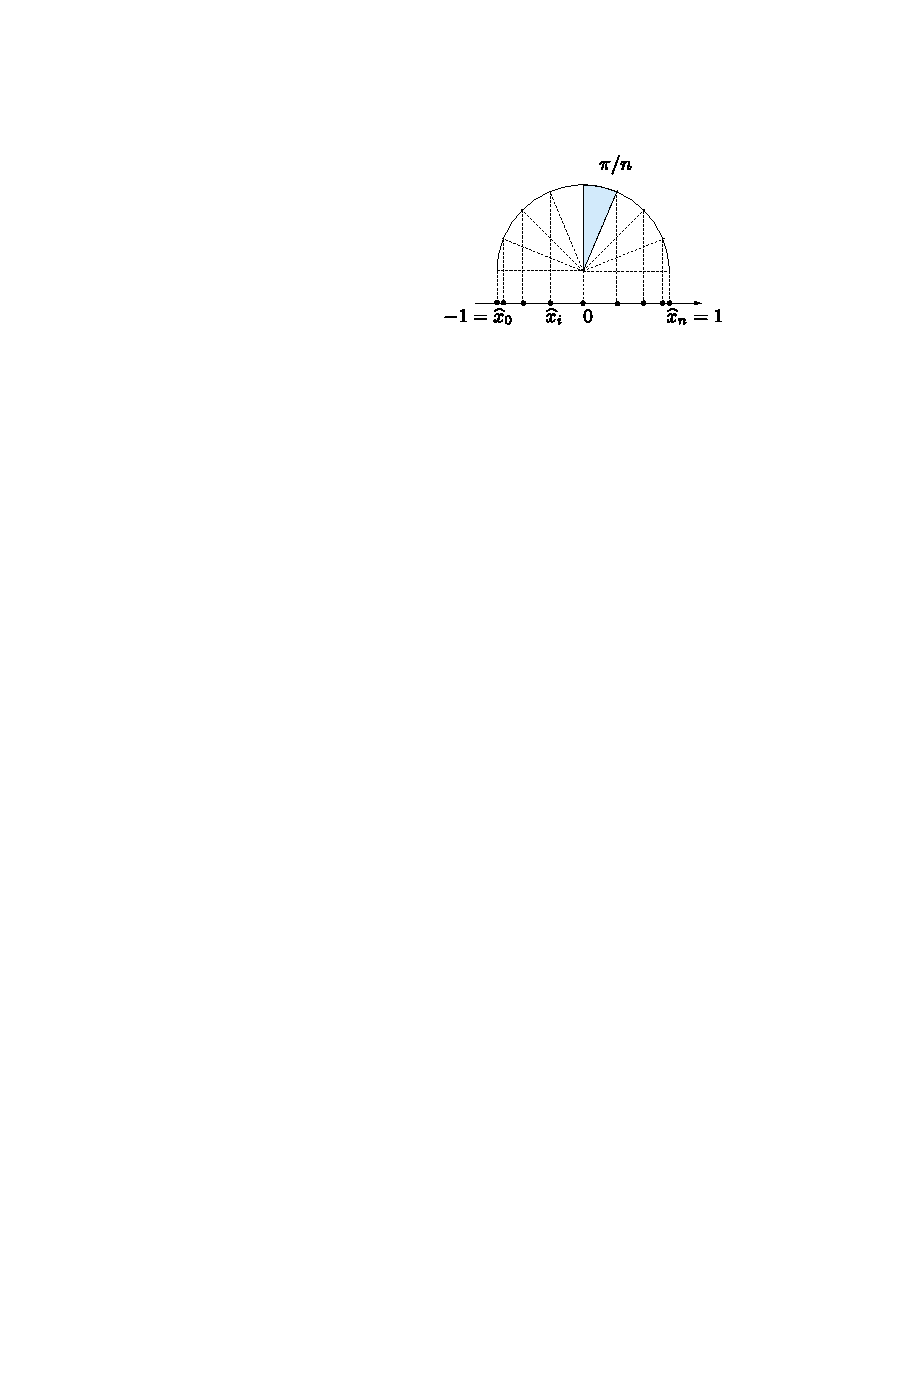
\includegraphics[width=.5\textwidth]{img/nodi-di-chebyshev-1.pdf}
	\caption{Distribuzione dei nodi di Chebyshev nell'intervallo $\left[-1, 1\right]$.}
\end{figure}

\noindent
Questi \definition{nodi di Chebyshev} sono \textbf{ottenuti come proiezioni sull'asse $x$ di punti sulla circonferenza unitaria individuati da settori circolari ottenuti con lo stesso angolo} $\frac{\pi}{n}$.

\highspace
\begin{flushleft}
	\textcolor{Green3}{\faIcon{question-circle} \textbf{E se viene applicato l'interpolatore Lagrangiano sui nodi di Chebyshev?}}
\end{flushleft}
Come detto all'inizio, si può modificare direttamente l'interpolatore Lagrangiano. Quindi, si consideri l'interpolatore Lagrangiano di grado $n$ costruito sui nodi di Chebyshev. Tale interpolatore si ottiene applicando le equazioni presentate precedentemente, con l'unico vincolo di \textbf{prendere in considerazione $\widehat{x}_{i}$ come nodi su cui costruire gli $n$ polinomi caratteristici di Lagrange}:
\begin{equation}
	\begin{array}{rcl}
		\widehat{\varphi}_{k}\left(x\right) &=& \displaystyle\prod_{j = 0, j \ne k}^{n} \dfrac{x - \widehat{x}_{i}}{\widehat{x}_{k} - \widehat{x}_{i}} \\ [1.5em]
		\displaystyle\prod_{n}^{C}\left(x\right) &=& \displaystyle\sum_{j=0}^{n} y_{j} \widehat{\varphi}_{j}\left(x\right)
	\end{array}
\end{equation}
La variabile $\prod_{n}^{C} \left(x\right)$ rappresenta l'\definition{interpolatore Lagrangiano sui nodi di Chebyshev}. Si indica con la rappresentazione $\prod_{n}^{C} f\left(x\right)$ quando viene applicato a dati ottenuti dalla valutazione di una funzione $f$, ovvero $y_{i} = f\left(x_{i}\right)$.

\longline

\subsubsection{Convergenza dell'interpolazione sui nodi di Chebyshev}

\begin{theorem}
	Si supponga che la funzione $f\left(x\right)$ ammetta derivata continua fino all'ordine $s+1$ compreso, ovverosia $f \in C^{\left(s+1\right)}\left(\left[-1,1\right]\right)$.
	
	\highspace
	Allora, si ha il seguente risultato di \definition{convergenza per l'interpolazione sui nodi di Chebyshev}:
	\begin{equation}
		\underset{x \in \left[-1,1\right]}{\max} \left|f\left(x\right) - \displaystyle\prod_{n}^{C} f\left(x\right)\right| \le \tilde{C} \dfrac{1}{n^{s}}
	\end{equation}
	Per un'opportuna costante $C$.
\end{theorem}

\noindent
Dal precedente teorema, si possono fare 3 osservazioni:
\begin{enumerate}
	\item Se $s \ge 1$ allora si è sicuri che ci sarà \textbf{sempre convergenza}:
	\begin{equation}
		\lim\limits_{n \rightarrow \infty} \underset{x \in \left[-1,1\right]}{\max} \left|f\left(x\right) - \displaystyle\prod_{n}^{C} f\left(x\right)\right| = 0
	\end{equation}
	
	\item La \textbf{velocità di convergenza aumenta all'aumentare di $s$}.
	
	\item \underline{Se} il teorema è valido $\forall s > 0$, allora la \textbf{velocità di convergenza è \emph{esponenziale}}. Questa è la migliore stima che è possibile ottenere, dato che è più veloce di qualsiasi altro $\frac{1}{n^{s}}$:
	\begin{equation}
		\underset{x \in \left[-1, 1\right]}{\max} \left| f - \displaystyle\prod_{n}^{C} f\left(x\right) \right| \le \tilde{C} e^{-n}
	\end{equation}
\end{enumerate}

\newpage

\subsubsection{Generalizzazione dell'intervallo}

Nel caso in cui il dominio di interesse non sia più da $\left[-1, 1\right]$ (come viene utilizzato nelle precedenti equazioni), ma un intervallo generale $\left[a,b\right]$, la \dquotes{conversione} può avvenire mappando i nodi $\widehat{x}_{j}$ da $\left[-1,1\right]$ a $\left[a,b\right]$:
\begin{equation}
	x = \psi\left(\widehat{x}\right) = \dfrac{a+b}{2} + \dfrac{b-a}{2} \: \widehat{x}
\end{equation}
Applicando la \definition{generalizzazione dell'intervallo ai nodi di Chebyshev}, si ottiene:
\begin{equation}
	x_{j}^{C} = \psi\left(\widehat{x}_{j}\right) = \dfrac{a+b}{2} + \dfrac{b-a}{2} \: \widehat{x}_{j} \hspace{2em} j = 0, \dots, n
\end{equation}
Di conseguenza, il \definition{polinomio di Lagrange applicato sui nodi di Chebyshev in un intervallo generale} diventa:
\begin{equation}
	\varphi_{k}^{C}\left(x\right) = \prod_{j = 0, j \ne k}^{n} \dfrac{x - x_{j}^{C}}{x_{k}^{C} - x_{j}^{C}}
\end{equation}
